\problemname{Linjen}

Dagens stadsplanering har brister.
Det krävs jättemånga bussar och spårvagnar för att driva ett kollektivtrafiknät.
Tänk om vi istället byggde en hel stad längs en linje?
Då skulle hela stadens transportbehov kunna tillgodoses med några få höghastighetståg.
Med denna briljanta idé byggdes en stad med $N$ tågstationer, var och en numrerad mellan $1$ och $N$.
För varje tågstation $i$ med $1 \leq i < N$, så finns det en tåglinje till tågstation $i+1$, som tar $1$ minut.
Varje linje kan tas i båda riktningarna.

Efter några år visar det sig att stadens form kanske inte är optimal.
Tack vare stadens välstånd har du som tur är utvecklat en teleportör.
Du ska installera den första teleportören och vill maximera dess påverkan.
Om du installerar teleportören mellan tågstationerna $i$ och $j$ kan du teleportera mellan tågstationerna i båda riktningarna.
Att teleportera tar en minut.
Det finns $K$ personer i staden.
Person $i$ bor i tågstation $s_i$ och arbetar i tågstation $t_i$.
Låt $\text{dist}(s,t)$ vara antalet minuter som den kortaste möjliga vägen mellan $s$ och $t$ tar,
som kanske eller kanske inte använder teleportören.

Om du installerar teleportören optimalt, vad är det minsta möjliga värdet av

$$\sum_{i=1}^{K} \text{dist}(s_i, t_i)$$

\section*{Indata}

Den första raden innehåller två heltal $N$ och $K$ ($1 \leq N \leq 10^9$, $1 \leq K \leq 10{,}000$),
antalet tågstationer och antalet personer.

De följande $K$ raderna innehåller vardera två heltal $s$ och $t$ ($1 \leq s,t \leq N$),
som betyder att det finns en person som bor i tågstation $s$ och arbetar i tågstation $t$.
Det är \textbf{inte} garanterat att alla par ($s,t$) är unika.

\section*{Utdata}
Skriv ut ett heltal: den minsta totala restiden om teleportören installeras optimalt.

\section*{Poängsättning}
Din lösning kommer att testas på en mängd testfallsgrupper.
För att få poäng för en grupp så måste du klara alla testfall i gruppen.

\noindent
\begin{tabular}{| l | l | p{12cm} |}
  \hline
  \textbf{Grupp} & \textbf{Poäng} & \textbf{Gränser} \\ \hline
  $1$    & $7$         & $N, K \leq 50$ \\ \hline
  $2$    & $14$        & $N, K \leq 500$ \\ \hline
  $3$    & $27$        & $N, K \leq 2000$ \\ \hline
  $4$    & $13$        & $N \leq 2 \cdot 10^5, K \leq 500$  \\ \hline
  $5$    & $18$        & $N \leq 2 \cdot 10^5, K \leq 2000$  \\ \hline
  $6$    & $21$        & Inga ytterligare begränsningar.  \\ \hline
\end{tabular}

\section*{Förklaring av exempelfall}
I exempelfall $1$ är det optimalt att bygga teleportören så att den enda invånaren kan ta sig till jobbet på en minut.

I exempelfall $2$ är en optimal lösning att bygga teleportören mellan tågstationerna $2$ och $9$.
I ritningen är varje persons hem kopplat med deras arbetsplats,
och den optimala teleportören är ritad som en streckad linje.

\begin{figure}[h]
  \centering
  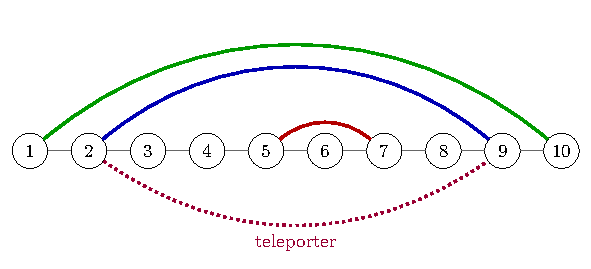
\includegraphics[width=0.7\textwidth]{sample2.pdf}
\end{figure}

Personen som bor i tågstation $1$ tar vägen $1 \rightarrow 2 \rightarrow 9 \rightarrow 10$,
personen i $2$ tar $2 \rightarrow 9$,
och personen i $5$ tar $5 \rightarrow 6 \rightarrow 7$.
Totalt tar detta $3+1+2=6$ minuter, vilket är optimalt.

I exempelfall $3$ är en optimal lösning att bygga en teleportör mellan tågstationerna $2$ och $9$.
